\documentclass{beamer}

\usepackage[utf8]{inputenc}
\usepackage[T2A]{fontenc}
\usepackage[english,russian]{babel}


\usepackage{tikz}
\usetikzlibrary{arrows,decorations.pathmorphing,backgrounds,fit,positioning,shapes,shapes.symbols,chains}

\usetheme{Metropolis}
\metroset{block=fill, numbering=fraction}

% Переведем заголовки блоков на русский
\uselanguage{russian}
\languagepath{russian}
\deftranslation[to=russian]{Claim}{Утверждение}
\deftranslation[to=russian]{Theorem}{Теорема}
\deftranslation[to=russian]{Example}{Пример}


% \usefonttheme{professionalfonts}
\usefonttheme{serif}
% \usefonttheme{structureitalicserif}


\DeclareMathOperator*{\argmin}{argmin}

\begin{document}

\title{Построение оптимального маршрута при заданной модели движения других участников транспортной сети}
\author{Разумова Л.Е., 610 группа\\Научный руководитель: к.ф.-м.н. Афонин С.А.}
\institute[]{Кафедра вычислительной математики}
\date[15.05.2022]{15 мая 2022}

% Создание заглавной страницы
% \frame{\titlepage}
\maketitle


% % Автоматическая генерация содержания
% \frame{
%   \frametitle{План}
%   \tableofcontents
% }

\section{Постановка задачи}

\begin{frame}\frametitle{Неформальная постановка}
  Рассматривается задача построения оптимального маршрута движения автотранспортного средства (АТС) при условии, что известны:
  \begin{itemize}
  \item дорожная сеть;
  \item время старта и маршруты движения других участников;
  \item правила, определяющие модель движения участников.
  \end{itemize}

  Маршруты других участников фиксированы. Скорость их движения определяется моделью движения. Задача состоит в прокладывании оптимального маршрута нового участника.
\end{frame}


\begin{frame}\frametitle{Сложность и новизна задачи}
  Маршруты движения участников могут пересекаться. Это приводит к изменению скоростного режима и образованию заторов.
  
  Традиционно, задачи прокладывания маршрута решают на основе статистического или исторического прогноза заторов (<<здесь каждое утро пробка>>). В данной работе мы считаем, что маршруты движения всех участников заранее известны.
\end{frame}


\begin{frame}\frametitle{Модель движения}
Дорожная сесть представляется ориентированным графом $ G = \langle V, E, l\rangle$, Вершины~--- перекрестки, ребра~--- дороги. Каждое ребро имеет длину, т.е. задана функция $l : E \rightarrow \mathbb {R} $.

  \textit{Моделью движения} АТС назовем $$M = \left(n, G, S, F, \{t_i\}_{i = 1}^n, \{\varphi_i\}_{i = 1}^n \right),$$ где $n$~--- количество участников движения, $G$~--- граф дорожной сети, $S$~--- множество состояний, которые могут принимать участники, $F \subset S$ --- множество заключительных состояний, $t_i: S^n \rightarrow R_{>=0}$ --- функция критического момента движения участника $i$, $\varphi_i: S^n \times \mathbb{R}_{>= 0} \rightarrow S$ --- функция перехода состояния $i$-ого участника в некоторый момент времени $t$.

\end{frame}


\begin{frame}\frametitle{Модель движения как автомат}
  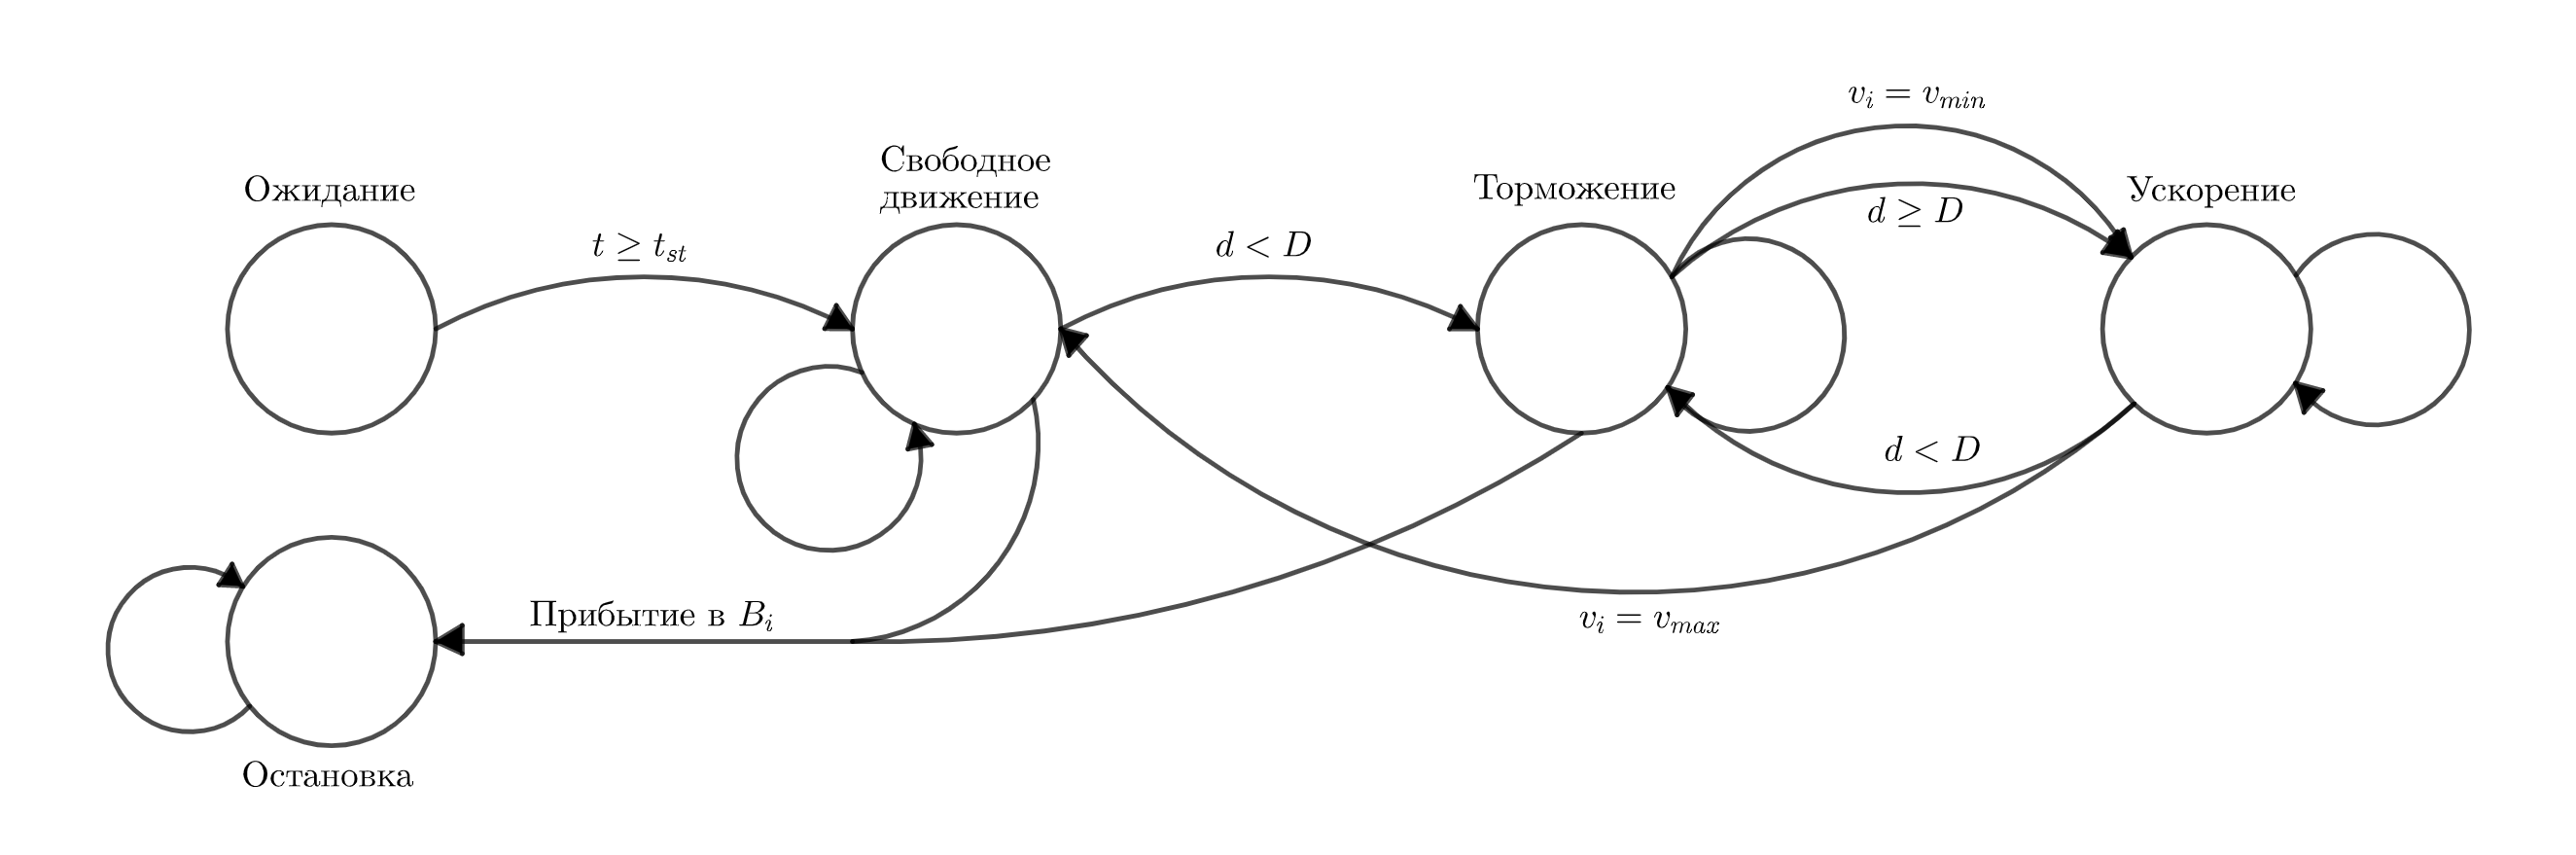
\includegraphics[width=\textwidth]{example-gen.png}
  Диаграмма для $i$-ого участника в модели движения, где $d$~--- расстояние до впереди идущего участника, $D$~--- максимальное расстояние взаимодействия с впереди идущим участником, $v_{max}$~--максимально возможная скорость, $v_{min}$~--минимально возможная скорость, $t_{st}$~-- время старта.
\end{frame}


\begin{frame}\frametitle{Задача прокладывания маршрута}
  Пусть $P(A,B)$ есть множество путей из $A$ в $B$ в графе $G$.
%  На множестве путей $P(A,B)$ определим $T(p) = \displaystyle \inf_t \{t : x_{n+1}(p, t) = 1\}$~-- время прибытия $(n+1)$-ого участника в вершину $B$ при движении по маршруту $p$. Требуется найти такой путь $p^* \in P(A, B)$, что $T(p^*)$ - минимальна. Другими словами,

  Для заданной модели движения $M = \left(n, G, S, F, \{t_i\}_{i = 1}^n, \{\varphi_i\}_{i = 1}^n \right)$ на графе дорожной сети $G=(V, E, l)$ при движении $n$ участников по путям $p_1, \dots, p_n$ требуется найти такой путь $p^*$ из $A$ в $B$, что движение нового участника по этому пути $p^*$ будет \textit{оптимально}, то есть
$$p^* = \argmin_{p \in P(A, B)} T(p),$$
где $T(p)$ есть время прибытия $(n+1)$-ого участника в вершину $B$ при движении по маршруту $p$ в соответствии с моделью $M$.
\end{frame}

\section{План решения}

\begin{frame}\frametitle{Кратчайший путь в динамическом графе}
  Рассматривается вспомогательная задача поиска пути в графе.
  
  Пусть на каждом ребре $e \in E$ графа $G(V, E)$ определена функция \textit{временных затрат} $\phi_e(t) : \mathbb {R}_+ \rightarrow \mathbb {R}_+$. Если мы оказались в начальной вершине ребра $e$ в момент времени $t$, то время преодоления ребра будет равняться $\phi_e(t)$.

  Задача состоит в нахождении пути $p^*$ с минимальной суммой $\sum_{e\in p^*}\phi_e(t)$.
\end{frame}

\begin{frame}\frametitle{Модифицированный алгоритм Дейкстры}

  Пусть $\mathcal{A}$~--- алгоритм Дейкстры поиска кратчайшего пути, в котором при посещении каждой вершины фиксируется время ее посещения и пересчитываются значения функции временных затрат на всех ребрах, исходящих из этой вершины.

  \begin{theorem}
    Если $$ \phi_e(t) \leq \Delta + \phi_e(t + \Delta), \quad \Delta \ge 0,$$
    то алгоритм $\mathcal{A}$ находит маршрут с минимальной суммой $\sum_{e\in p^*}\phi_e(t)$.
  \end{theorem}
\end{frame}

\begin{frame}\frametitle{Построение функций $\phi_e(t)$}
  Значения функций временных затрат $\phi_e(t)$ получаются в процессе симуляции движения АТС согласно модели движения
  $$M = \left(n, G, S, F, \{t_i\}_{i = 1}^n, \{\varphi_i\}_{i = 1}^n \right).$$

  Для состояния $S$ в момент $t$ вычисляется ближайший критический момент $t'=\min\limits_{i\in\{1,\ldots,n\}} t_i(S)$. На промежутке $[t, t']$ движение вычисляется по известным формулам, далее производится изменение состояния и вычисляется следующий критический момент.
\end{frame}

\section{Результаты численных экспериментов}

\begin{frame}\frametitle{Модель следования за лидером}
  В рамках численных экспериментов была реализована модель следования за лидером, определенная правилами, представленными на диаграмме.
  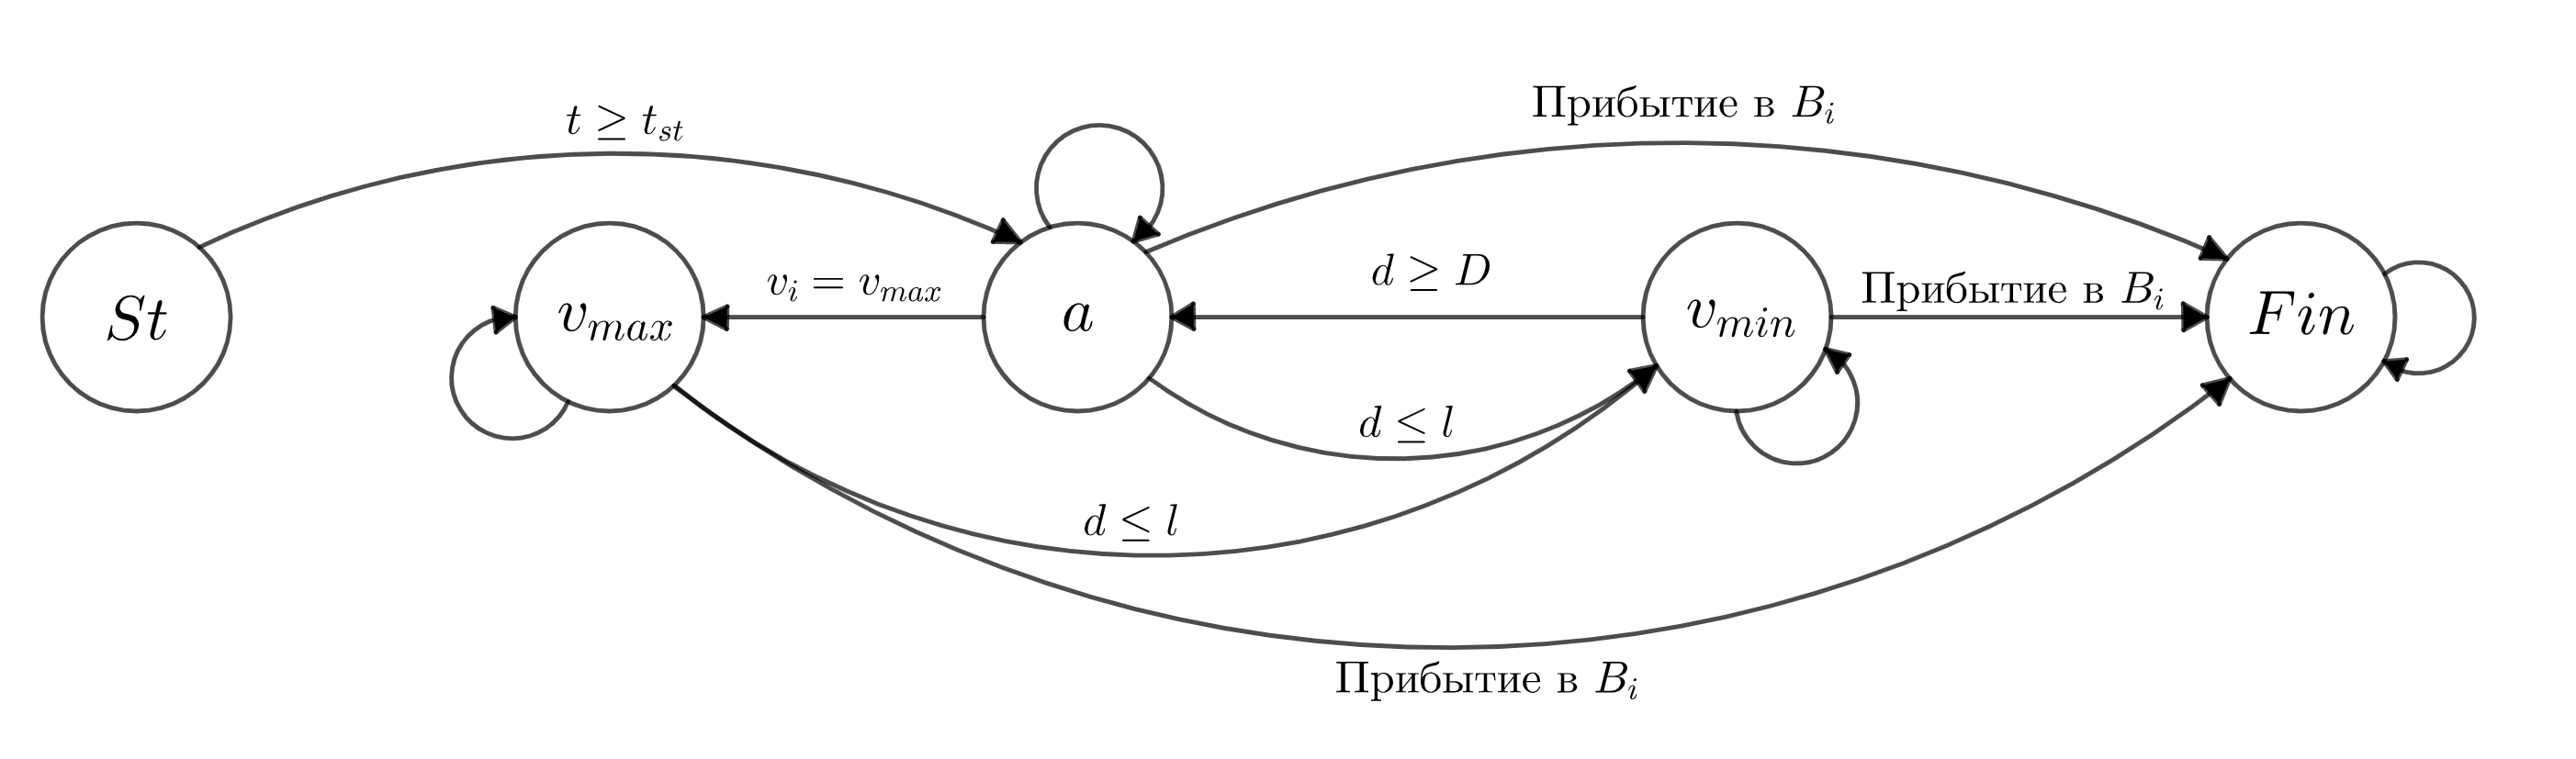
\includegraphics[width=\textwidth]{Micro-gen.png}
  Параметры модели: \\
  \begin{itemize}
  	\item Безопасное расстояние $D$, дистанция торможения $l$
  	\item Максимальная $v_{max}$, минимальная $v_{min}$ скорости и ускорение $a$
  	\item Время старта $t_{st}$
  \end{itemize}
\end{frame}


\begin{frame}\frametitle{Результаты моделирования}
	\begin{center}
		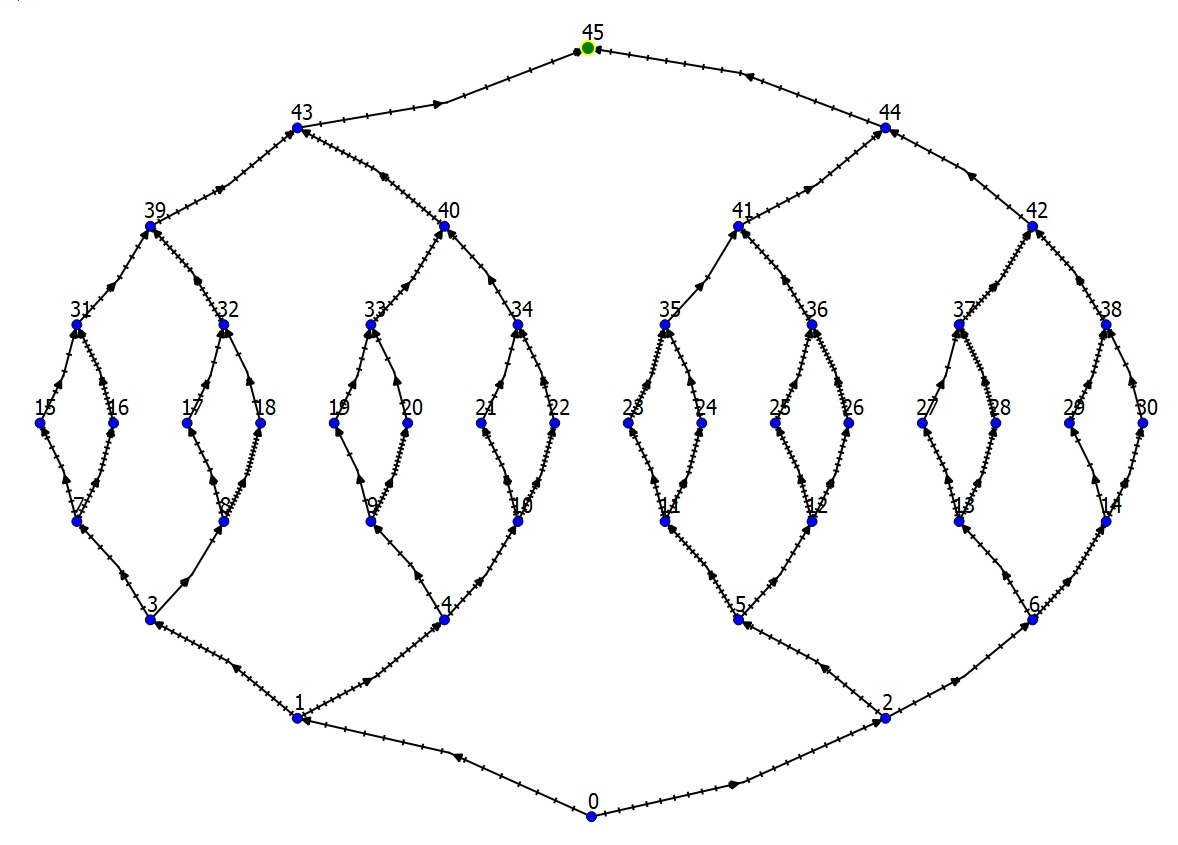
\includegraphics[scale=0.2]{Graph_N.jpg}
	\end{center}
   
   Граф дорожной сети $G$, на котором производилось моделирование движения. $|V| = 46, \; |E| = 60$, ребра произвольной длины.
\end{frame}

\begin{frame}\frametitle{Результаты моделирования}
	Были получены результаты:
	\begin{table}[H]
		\label{tab:res_average}
		\centering
		\begin{tabular}{|c|c|c|c|c|}
			\hline
			\multicolumn{1}{|c|}{ $t_{st}$} & $v_{max}$  & $v_{min}$ & $a$ &  $T(p^*)$ \\ \hline
			\multicolumn{1}{|c|}{$5$}       & 60         & 10        & 4.375 &   955.321         \\ \hline
			\multicolumn{1}{|c|}{$5$}       & 60         & 20        &  4   &     935.259        \\ \hline
			\multicolumn{1}{|c|}{$5$ }      & 80         & 10        &  7.875   &    716.872         \\ \hline
			\multicolumn{1}{|c|}{$5$}       & 80 & 20                  & 7.5 &        707.094           \\ \hline
			\multicolumn{1}{|c|}{$40$}      & 60 & 10                  & 4.375    &  1172.52            \\ \hline
			\multicolumn{1}{|c|}{$40$ }     & 60 & 20                  & 4   &       1083       \\ \hline
			\multicolumn{1}{|c|}{$40$}      & 80 & 10                  & 7.875    &    906.91          \\ \hline
			\multicolumn{1}{|c|}{$40$ }     & 80 & 20                  & 7.5   &       864.625       \\ \hline
			
		\end{tabular}
		\caption{Результаты запуска модифицированного алгоритма Дейкстры. В таблце представлены значения времени на прохождение оптмального пути с параметрами $v_{max}, \; v_{min}, \; a = \frac{v^2_{max}-v^2_{min}}{2(D-l)}$.}
	\end{table}
\end{frame}


\begin{frame}\frametitle{Выводы}
  \begin{itemize}
  \item Предложена автоматная форма определения модели движения АТС.
  \item Разработан и реализован алгоритм симуляции движения АТС в соответствии с заданной моделью движения.
  \item Сформулировано необходимое условие, при котором модифицированный алгоритм Дейкстры приводит к нахождению оптимального решения.
  \item Показано, что для модели следования за лидером возможно отклонение найденного решения от оптимального.
  \end{itemize}
\end{frame}


\begin{frame}[standout]
Спасибо за внимание!
\end{frame}


\end{document}
